%%%%%%%%%%%%%%%%%%%%%%%%%%%%%%%%%%%%%%%%%

%%%%%%%%%%%%%%%%%%%%%%%%%%%%%%%%%%%%%%%%%

%----------------------------------------------------------------------------------------
%	PACKAGES AND DOCUMENT CONFIGURATIONS
%----------------------------------------------------------------------------------------

\documentclass{article}
\usepackage{siunitx} % Provides the \SI{}{} command for typesetting SI units
\usepackage{graphicx} % Required for the inclusion of images
\usepackage[square, numbers, comma, sort&compress]{natbib}
\usepackage{caption} 
\usepackage[section]{placeins}
\captionsetup[table]{skip=10pt}
\setlength\parindent{0pt} % Removes all indentation from paragraphs
% \newgeometry{margin=-1cm}
% \addtolength{\oddsidemargin}{-.275in}
% \addtolength{\evensidemargin}{-.275in}
% \addtolength{\textwidth}{1.75in}
% 
% \addtolength{\topmargin}{-.275in}
% \addtolength{\textheight}{1.75in}


%----------------------------------------------------------------------------------------
%	DOCUMENT INFORMATION
%----------------------------------------------------------------------------------------

\title{Molecular Dynamics Simulation \\ of Argon \\ for AP3081 D} % Title

\author{Bas \textsc{Nijholt}} % Author name

\date{\today} % Date for the report

\begin{document}

\maketitle % Insert the title, author and date

\begin{center}
\begin{tabular}{l r}
Date started: & February 3, 2014 \\ 
Instructor: & Dr. J.M. Thijssen
\end{tabular}
\end{center}

% If you wish to include an abstract, uncomment the lines below
\begin{abstract}
Molecular Dynamics simulation is a technique for computing equilibrium and dynamic properties of a classical many-body system. Newton’s equations of motion are solved numerically, and macroscopic properties of the system are measured by applying statistical mechanics principles. In this report, we will discuss the key ingredients in carrying out a molecular dynamics simulation. This includes the potentials used to model intermolecular interactions, the integration algorithms and the boundary conditions that are implemented. We will present the results of simulations performed for a system of 864 particles interacting through a Lennard\text{-}Jones potential, and interpret the results for argon.
\end{abstract}

%----------------------------------------------------------------------------------------
%	SECTION 1
%----------------------------------------------------------------------------------------

\section{Introduction}
With computer simulation we study macroscopic systems which can not be solved analytically. This is done by implementing microscopic models which specify intermolecular interactions and molecular structure.
The result from computer simulations can be compared with analytical predictions and experimental data to test the accuracy of the model. Molecular dynamics uses computer simulation with statistical mechanics to compute static and dynamic properties of a classical many-body system. Static properties include the energy, temperature and pressure of a system while dynamic properties include the diffusion coefficient and time correlation functions of a system. In our molecular dynamics simulations we first specify the initial positions and momenta of the particles. Then we evolve the system according to Newton’s second law: $ F_{i} = m_{i} \cdot a_{i}$ in which we let the particles interact through a Lennard\text{-}Jones potential.
Finally we measure physical quantities as functions of particle positions and momenta.
Statistical mechanics is used to interpret the static properties such as temperature and pressure.
The results obtained from the simulations are interpreted for argon for which the Lennard\text{-}Jones description has been very successful \citep{PhysRev.136.A405}.
With our assay we aim to study macroscopic systems, but only a "small" finite number of particles can be simulated on a computer.
Real systems contain $\mathcal{O}(10^{23})$ particles \footnote{Avogadro's constant is $6.022\cdot 10^{23} \; \si{\per\mole}$}. 
To mimic the bulk surrounding the sample, periodic boundary conditions are implemented.
This and other considerations in setting up a molecular dynamics simulation, such as the integration algorithms are discussed in Chapter 2. 
In Chapter 3, results of computer simulations are presented. 
We will compare these results to the simulations done by Verlet in 1967 \citep{PhysRev.159.98}. His data corresponds very well to experimental data \citep{Levelt1960361, VanItterbeek1963742, Michels1949627}.


\subsection{Intermolecular Interactions}
The intermolecular interactions are modeled by the 12-6 Lennard\text{-}Jones potential as in figure \ref{fig:LJ}, which is typically used to model interactions between non-polar molecules. This potential is a function of the positions of the nuclei and depends only on the magnitude of the pair separation $r_{ij}= \left| \mathbf{r}_i - \mathbf{r}_j \right|$. We will only consider these pairwise interactions, since their contribution is most significant. The potential energy of the whole system is written as
\begin{equation}
\label{pot}
 U\left(  \mathbf{r}^N \right) = \sum_{i} \sum_{i<j} \phi_{LJ}(r)
\end{equation}
in which the Lennard\text{-}Jones potential $\phi_{LJ}$ is
\begin{equation}
 \phi_{LJ}(r) = 4\epsilon \left[  \left(  \frac{\sigma}{r}\right)^{12} - \left(  \frac{\sigma}{r}\right)^{6} \right]
\end{equation}


\begin{figure}[!htb]
  \centering
    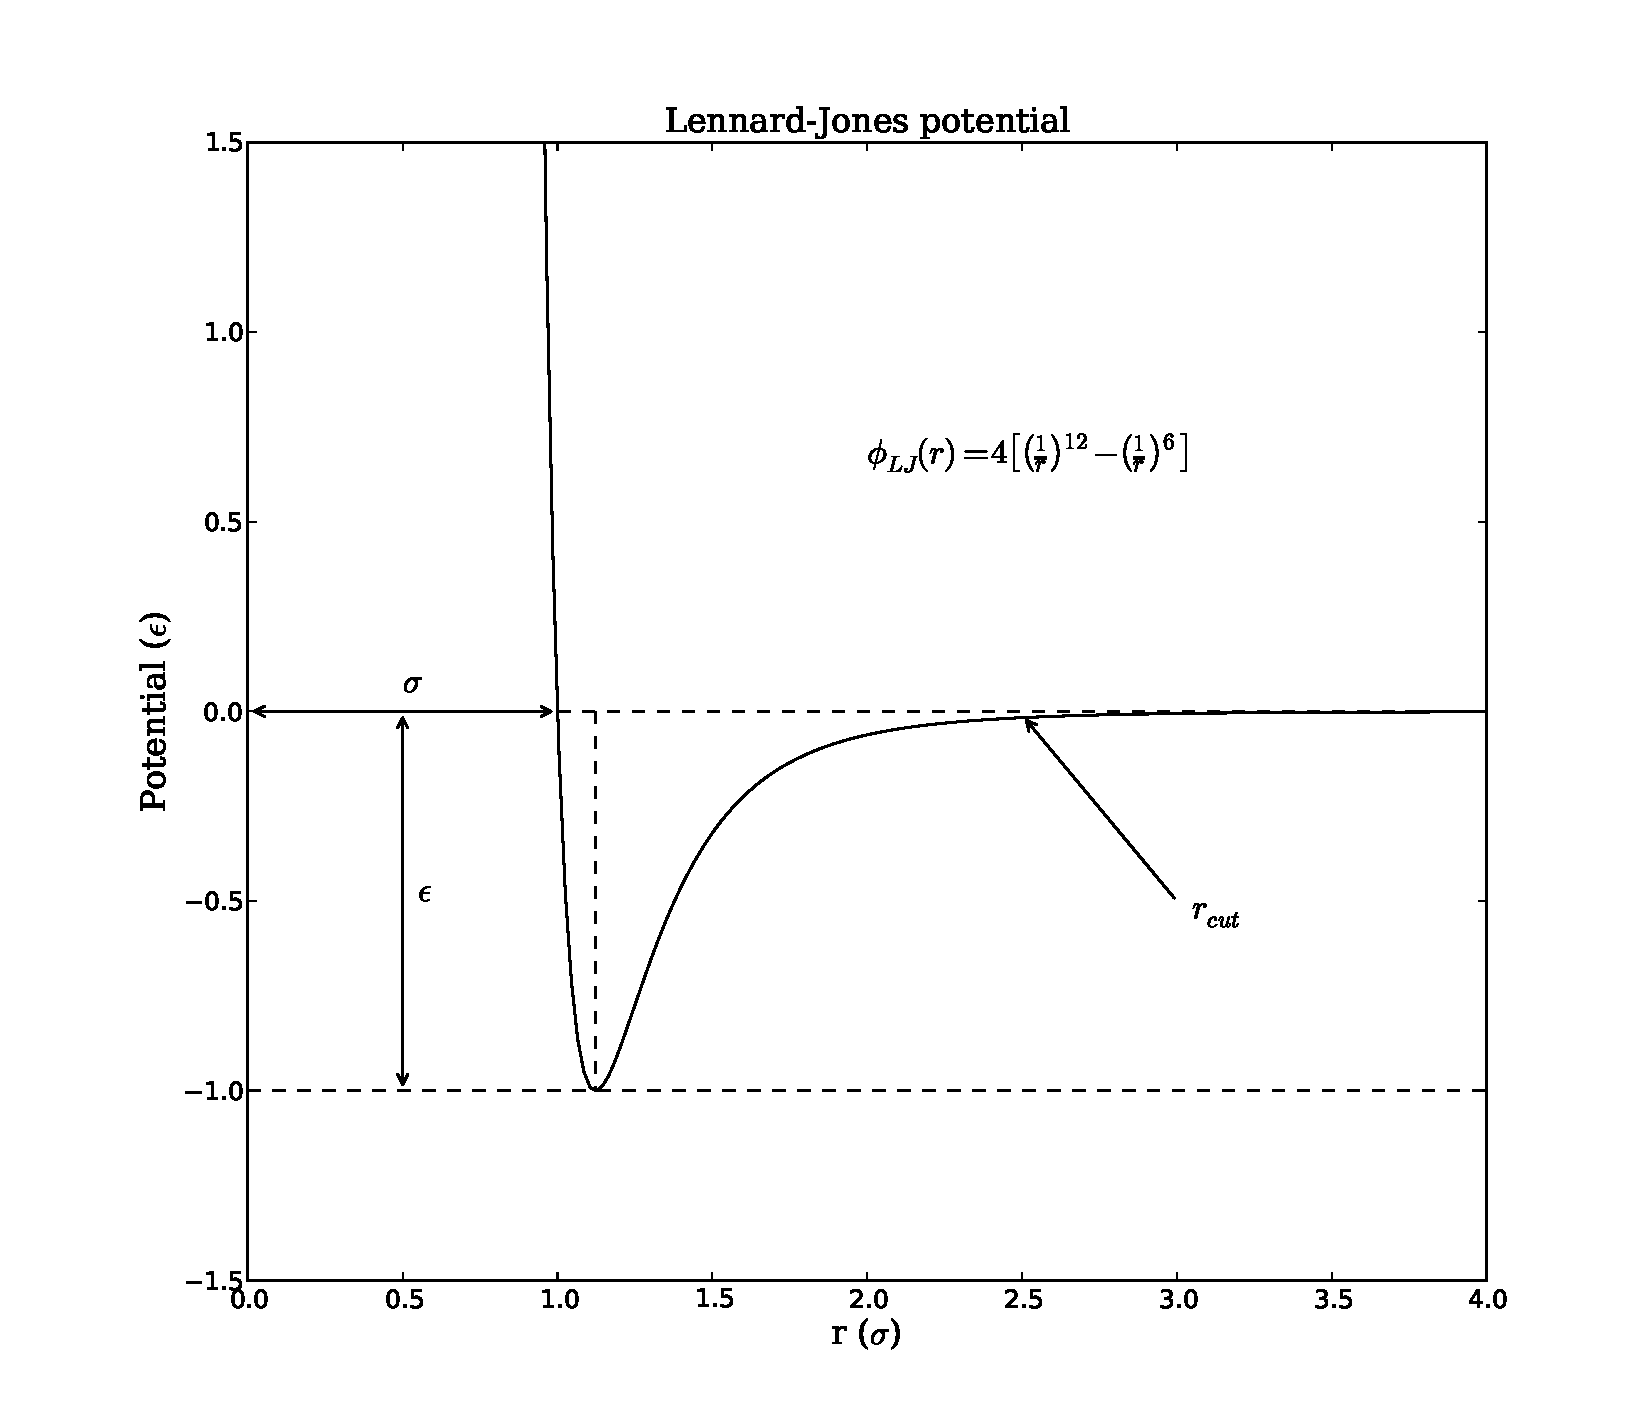
\includegraphics[height=100mm]{LJ.pdf}
  \caption[]{A graph of strength versus distance for the 12-6 Lennard\text{-}Jones potential with $\sigma=\epsilon=1$ in which the significant parameters are depicted. The potential in cut at $r_{cut}=2.5 \sigma$ which is explained in the computation part of the report.}
  \label{fig:LJ}
\end{figure}

Here $\sigma$ represents the effective diameter of the spherical particles and $\epsilon$ measures the attractive interaction as is indicated in figure \ref{fig:LJ}. The potential consists of a short-range repulsive force ($1/r^{12}$) arising from screening effects and from Pauli's exclusion principle, and a long-range attractive force ($1/r^6$) arising from van der Waals dispersion forces. In this report we choose $\sigma=\epsilon=1$. The total intermolecular force is the gradient of the potential with respect to particle displacements.

\begin{equation}
\label{forcegrad}
 \mathbf{F}_i=-\sum_{i\neq j} \frac{\partial \phi_{LJ}(r_{ij})}{\partial r_{ij}}=-24 \sum_{i\neq j}  \left[ 2 \left(  \frac{1}{r_{ij}}\right)^{13} - \left(  \frac{1}{r_{ij}}\right)^{7} \right]
\end{equation}

\subsection{Boundary Conditions}
Though we try to find information about a physical system, only a small number of particles is considered, while a real physical system contains many moles of particles $\mathcal{O}(10^{23})$ which is impossible to simulate exactly. Because we choose a system of 'only' 864 particles, the ratio of surface molecules to the molecules in bulk is higher than in reality. Therefore periodic boundary conditions are implemented, which mimics the behavior of the infinite bulk surrounding the sample. In this way surface effects are removed. In figure \ref{fig:BC} one can see the difference in using a periodic or a hard wall boundary condition. It should also be noted that if the particles go through the wall, they will appear at the other side of the box.

\begin{figure}[!htb]
  \centering
    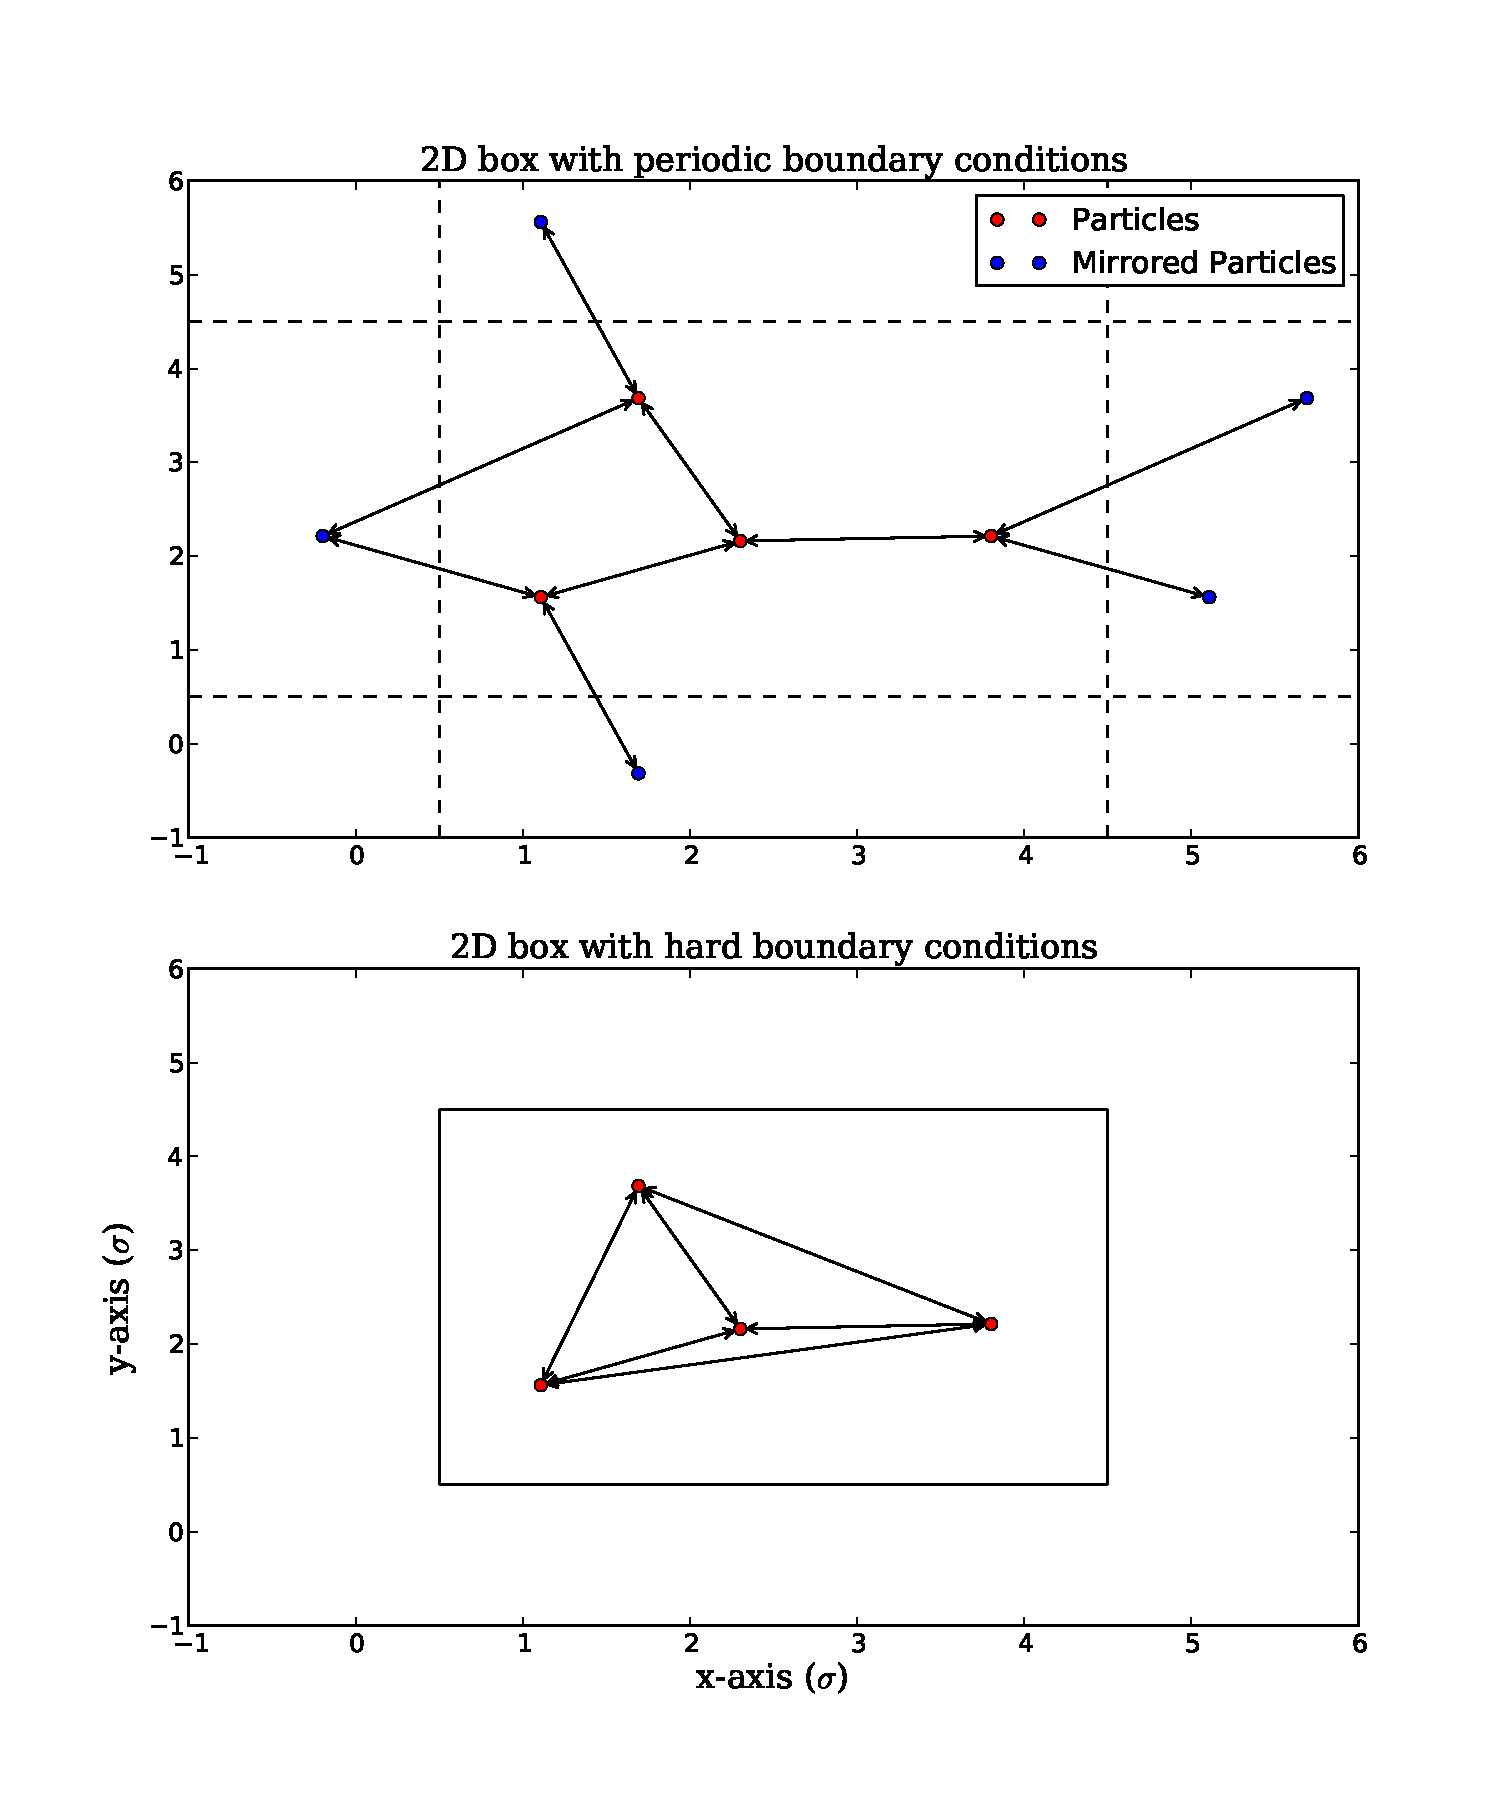
\includegraphics[height=130mm]{BC.pdf}
  \caption[]{The choice of the type of boundary conditions (BCs) affects the properties of the system that is considered. In the figure hard walls and periodic BCs are compared. The top graph represents a two-dimensional system with periodic BCs and the graph at the bottom has hard walls as BCs. The arrows represent the pairwise interaction between two atoms. In the case of the periodic BCs, the nearest atom might not lie in the box itself, but an atom in a adjacent box (its mirror image) could be closer .}
  \label{fig:BC}
\end{figure}

\subsection{Nearest\text{-}Neighbor Interaction}
Using periodic boundary conditions solves the problem of surface effects, but gives rise to a new difficulty. Namely, we have $N=864$ particles in a box, those particles do not only interact with each other, but also interact with particles in the periodic (mirrored) images. The short-range interactions of the Lennard\text{-}Jones potential are dominated by the interactions of the particles closer than a cut-off distance $r_{cut}$, as is indicated in figure \ref{fig:LJ}. We choose a cut-off radius such that $r_{cut} \le \frac{1}{2}L_{box}$. So the truncated potential becomes:

\begin{equation}
 U(r)=\left\{
\begin{array}{c l}      
    \phi_{LJ}(r), & r \le r_{cut}\\
    0 & r>r_{cut}
\end{array}\right.
\end{equation}

\subsection{Equations of Motion}
The classical equations of motion for the $i$th particle can be written as
\begin{equation}
m_i\ddot {\vec x}_i(t)=F_i(\vec x(t))=-\nabla_{\vec x_i} \phi(\vec x(t))\end{equation}
in which $t$ is the time, $\vec x(t)=(\vec x_1(t),\ldots,\vec x_N(t))$ is the ensemble of the position vector of $N$ particles, $F$ is the force and $\phi$ is the scalar potential function, which is the Lennard\text{-}Jones potential in our case.\\

We can use finite difference methods to solve these differential equations approximately. In this report Verlet's velocity scheme is used, where positions, velocities and acceleration at time $t+\Delta t$ are obtained from the same quantities at time $t$ in the following way:



\begin{equation}
\label{verlet1}
\vec{x}(t + \Delta t) = \vec{x}(t) + \vec{v}(t)\, \Delta t + \frac{1}{2} \,\vec{a}(t) \Delta t^2  \,
\end{equation}


\begin{equation}
\label{verlet2}
\vec{v}(t + \Delta t) = \vec{v}(t) + \frac{\vec{a}(t) + \vec{a}(t + \Delta t)}{2} \Delta t  \,
\end{equation}

\subsection{Reduced Units}
\label{reduced}
In this report physical quantities are expressed as dimensionless or natural (reduced) units. This means that all quantities of interest are put to unity, so we do not work with very large or very small numbers. An advantage is that the equations of motion become simplified.\\

The following basic units are put to unity:
\begin{center}
\begin{itemize}
 \item length: $\sigma=\SI{3.405}{\angstrom}$ for argon
 \item energy: $\epsilon=\SI{119.8}{\degree\kelvin}$ for argon
 \item mass: $m=39.9$ amu for argon\footnote{one amu is \SI{1.66053892e-27}{\kilogram}}
 \item Boltzman's constant: $k_B=\SI{1.381e-23}{\joule\per\kelvin}$
\end{itemize}
\end{center}

Other derived reduced quantities are time $t^*=t\sqrt{\epsilon/m\sigma^2}$, pressure $P^*=P\sigma^3/\epsilon$, temperature $T^*=k_bT/\epsilon$, and density $\rho^*=\rho^3$.\\

For simplicity we will indicate the unit of time as $\Delta t$.
 
%----------------------------------------------------------------------------------------
%	SECTION 2
%----------------------------------------------------------------------------------------

\section{Computer Simulation}
The simulations were constructed as follows:
\begin{enumerate}
 \item Initialize particle positions and momenta.
 \item Compute forces on particles.
 \item Integrate equation of motion.
 \item Measure relevant quantities.
 \item Repeat (2)\text{-}(4) for the designated period of time.
 \item Compute averages.
\end{enumerate}

\subsection{Initialization}
The particles are initiated at positions such that there is no overlap of the atomic cores. An easy way of doing this is placing the atoms on a lattice. For the simulations done in this report, we chose to place them on a face-centered cubic lattice for close packing as in figure \ref{fig:lattice}. The lattice spacing was chosen to obtain the desired particle density. 

\begin{figure}[!htb]
  \centering
    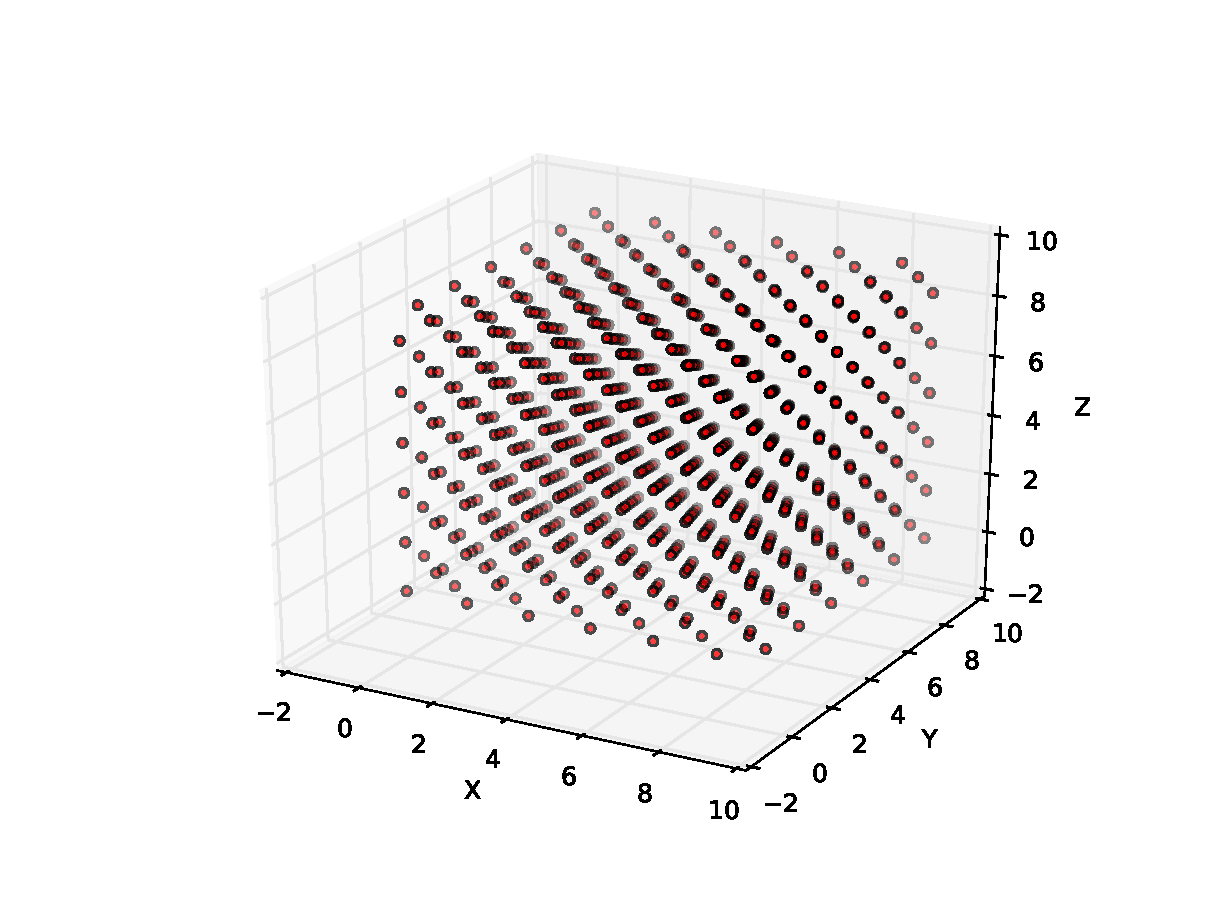
\includegraphics[height=80mm]{fcc.pdf}
  \caption[]{The atoms are initialy placed on a face-centered cubic lattice (FFC). The atom positions in the figure are depicted by the red points.}
  \label{fig:lattice}
\end{figure}

The initial velocities must satisfy the desired initial temperature\footnote{Temperature and velocity are related as $\frac{1}{2}mv^2=\frac{3}{2}k_B T$}. They can be arbitrarily selected from the Maxwell-Boltzmann distribution

\begin{equation}
  f(v) = \sqrt{\left(\frac{m}{2 \pi kT}\right)^3}\, 4\pi v^2 \exp \left(- \frac{mv^2}{2kT}\right), 
\end{equation}

In order to generate normally distributed numbers from uniformly distributed random numbers the Box-Muller transform is used

\begin{equation}
 Z_0 = R \cos(\Theta) =\sqrt{-2 \ln U_1} \cos(2 \pi U_2)\,
\end{equation}

in which $U_1$ and $U_2$ are uniformly distributed random numbers. The initial velocities that are generated have a very similar distribution as in the end of the simulation. This can be seen in figure \ref{fig:velocity_ic}, which also justifies the use of the Maxwell-Boltzmann distribution.

\begin{figure}[!htb]
  \centering
    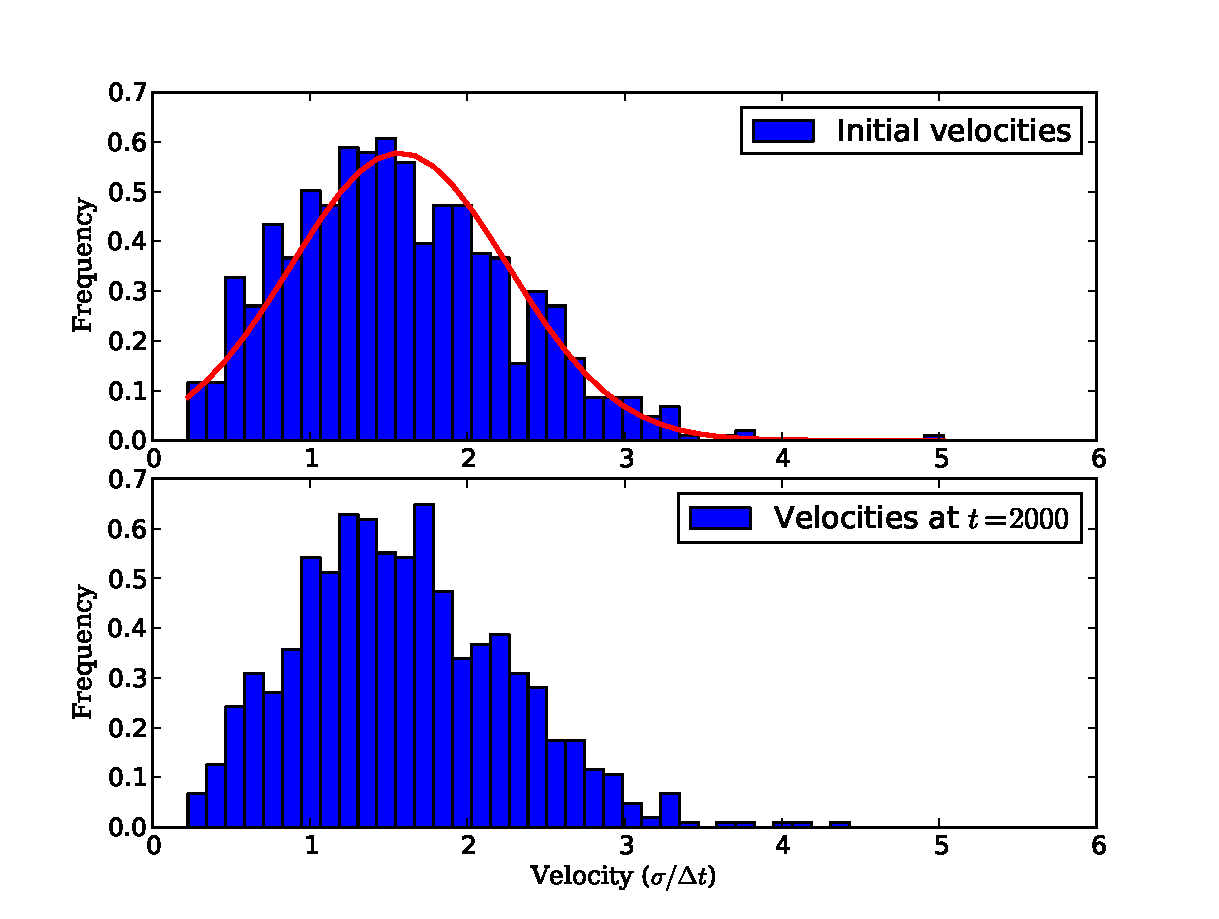
\includegraphics[height=80mm]{velocity_ic.pdf}
  \caption[]{The initial velocities of the atoms are normally distributed (top histogram). The red curve is a Gaussian fit. After the simulation is done the distribution is still normally distributed (lower histogram).}
  \label{fig:velocity_ic}
\end{figure}

\subsection{Computing Forces}
The force is the gradient of the Lennard\text{-}Jones potential (equation \ref{forcegrad}). So the force of the $x$-component on the $i$th particle is given by

\begin{equation}
 f_{x_i}(r) = - \frac{\partial \phi_{LJ}(r)}{\partial x_i}
 = - \left( \frac{x_i}{r} \right) \left( \frac{\partial \phi_{LJ}(r)}{\partial r} \right)
 =\frac{48x_i}{r^2} \left[ \frac{1}{r^{12}} - 0.5\frac{1}{r^6} \right]
\end{equation}

\subsection{Integration}
We implemented Verlet's velocity scheme (equations \ref{verlet1} and \ref{verlet2}) as follows:

\begin{enumerate}
 \item calculate $\vec{v}\left(t + \Delta t \right) = \vec{v}(t) + \frac{1}{2} \vec{a}(t)\Delta t$
 \item calculate $\vec{x+\Delta t}(t) = \vec{x}(t)+\vec{v}(t+ \Delta t)\Delta t \pmod{L_{box}}$
 \item derive $\vec{a}(t + \Delta t)$ from the interaction potential using $\vec{x}(t+\Delta t)$
 \item calculate $\vec{v}\left(t + \Delta t \right) = \vec{v}(t+\Delta t) + \frac{1}{2} \vec{a}(t+\Delta t)\Delta t$
\end{enumerate}

A time-step of $\Delta t = 0.004$ is used, unless indicated differently.

\subsection{Measurements}
The system must establish equilibrium before measurements can be made. The temperature is rescaled with a factor $\sqrt{T/T_{0}}$ for a certain time until the desired temperature ($T_0$) is reached as is shown in figure \ref{fig:equil}. After equilibrium is reached, the total energy is constant as can be seen in figure \ref{fig:energies}. \\

\begin{figure}[!htb]
  \centering
    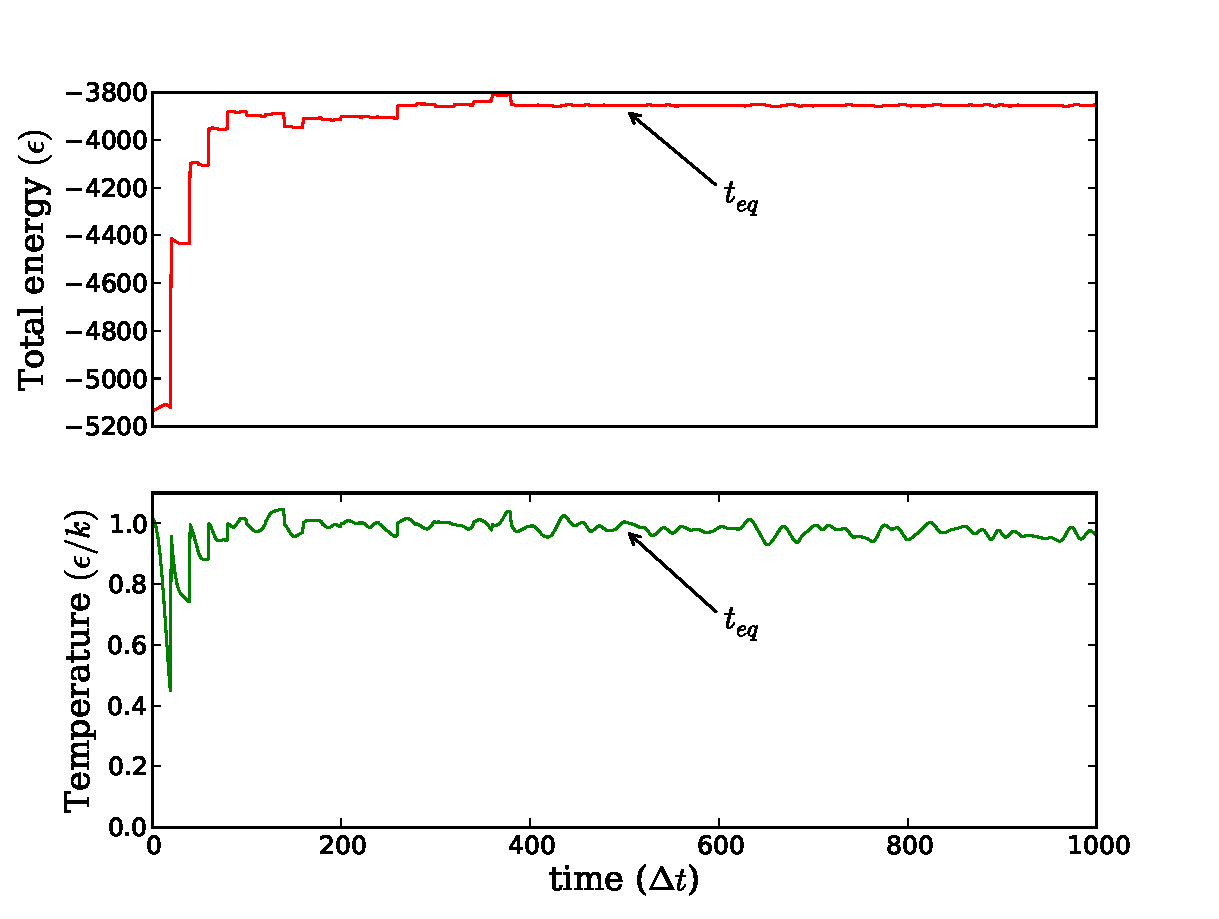
\includegraphics[height=80mm]{equil.pdf}
  \caption[]{The temperature is rescaled every 20 time-steps until $t_{eq}$, which in this case $t_{eq}=500$. We then assume the total energy constant. This system has a density $\rho=0.85$.}
  \label{fig:equil}
\end{figure}


\begin{figure}[!htb]
  \centering
    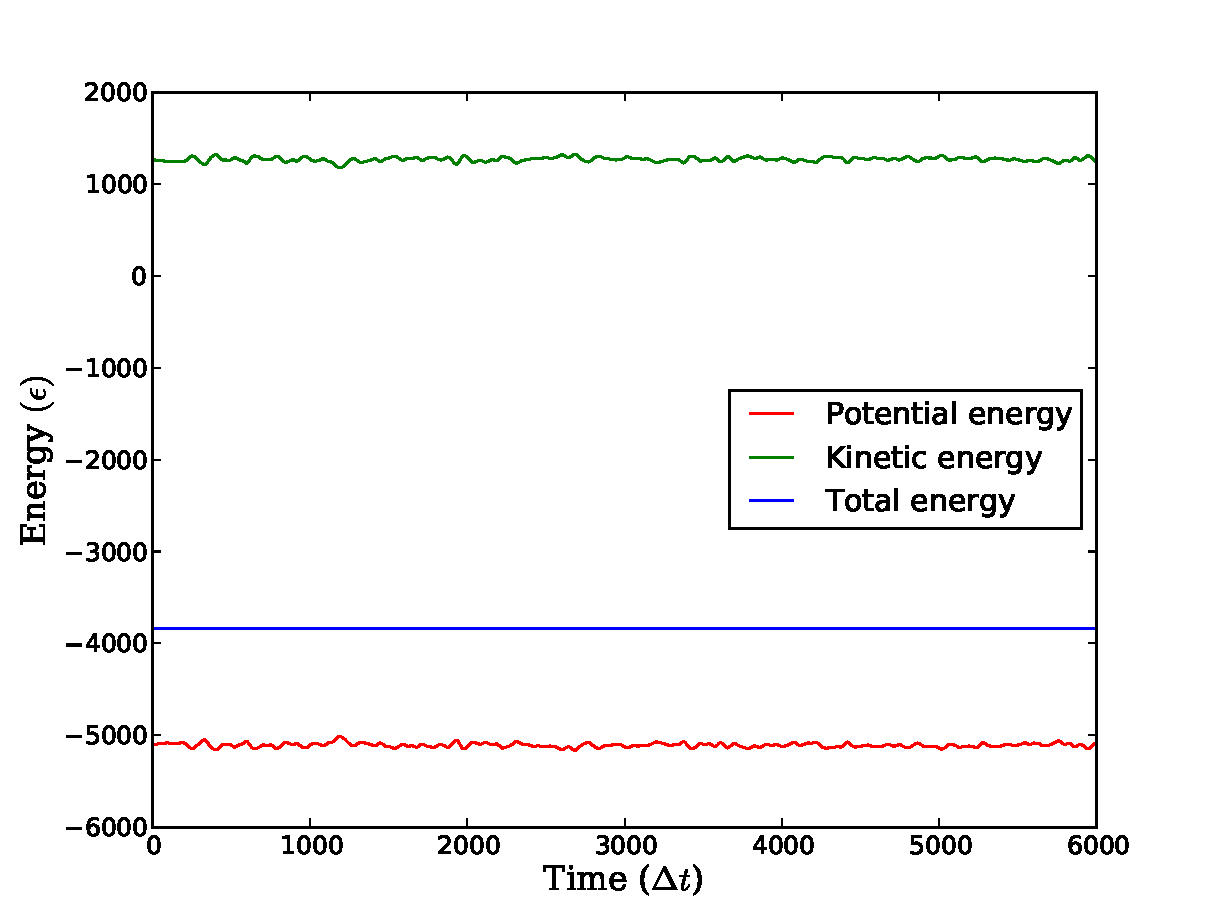
\includegraphics[height=80mm]{energies.pdf}
  \caption[]{Equilibration phase for a system at $T = 1$ and $\rho = 0.85$. The potential and kinetic energy fluctuate about equilibrium values while the total energy is practically constant.}
  \label{fig:energies}
\end{figure}

The measurements involve time averages of a physical quantity $A$ over the system trajectory

\begin{equation}
 \left\langle  A \right\rangle = \frac{1}{N} \sum_{i=1}^N A_i(t)
\end{equation}
for $N$ time-steps. The values $A_i(t)$ are considered as independent if one correlation time $\tau$ has past. The correlation time $\tau$ is found by calculating the auto-correlation function as in figure \ref{fig:auto_correlation}. The correlation time is defined as the time it takes for the autocorrelation function to have a factor of $1/e$ of its original value. The correlation time is $5 < \tau <25$ depending on the system, so for safety $\tau=50$ is used. \\

\begin{figure}[!htb]
  \centering
    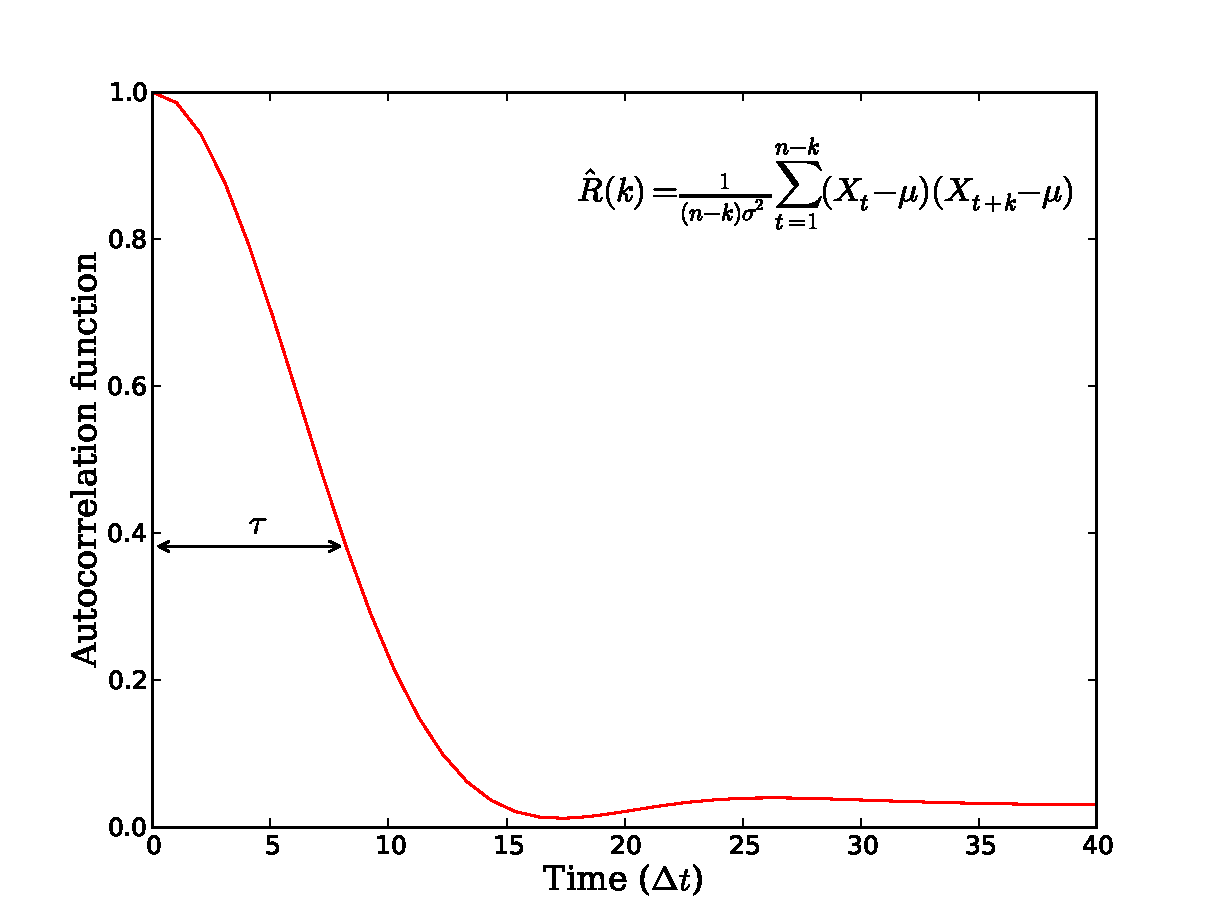
\includegraphics[height=80mm]{auto_correlation.pdf}
  \caption[]{Time dependence of the estimated autocorrelation function. The correlation time $\tau$ is indicated, which is about 8 in this case.}
  \label{fig:auto_correlation}
\end{figure}

The averages are subject to systematic and statistical errors. Systematic errors are associated with numerical integration, finite size effects and the interaction cut-off. Statistical errors are due to random fluctuations in measurements. To make the values $A_i$ values independent, block averaging \citep{blockavg} is used. Which means that the average over blocks of 50 successive values is taken and used to calculate the variance, so the variance of the averages gives a measure of the error. \\

The following physical properties were measured:\\ \\

\textbullet \textbf{ Energy: } The total energy in each time-step is measured. The total energy $E=K(t)+U(t)$ is conserved by classical Newtonian dynamics (figure \ref{fig:energies}). The potential energy $U(t)$ is given by equation \ref{pot} and the kinetic energy is

\begin{equation}
 K(t)=\frac12 \sum_{i=1}^N \left| v_i(t) \right|^2
\end{equation} \\ \\


\textbullet \textbf{ Temperature: } The instantaneous temperature is computed from the equipartition theorem which states that the kinetic energy equals $\frac12 N k_B T$ per degree of freedom. In the case of argon

\begin{equation}
 K = \frac32 N k_B T
\end{equation} \\ \\ 


\textbullet \textbf{ Pressure: } The pressure can be found in a simulation using the virial theorem \citep{virial,thijssen2007computational, PhysRev.159.98}:

\begin{equation}
 \frac{\beta P}{\rho}=1-\frac{\beta}{3N}\left\langle \sum_{i=1}^N \vec{r}_i\nabla_i \phi_{LJ}(r) \right\rangle
\end{equation} 
where $\left\langle \cdots \right\rangle$ denotes the time average and $\beta=1/k_B T$. As the potential is truncated at $r_{c}=2.5$, a correction term is needed. The correction term is proportional to

\begin{equation}
-\frac{2\pi N \rho}{3k_BT} \int_{r_{c}}^{\infty} \frac{\partial \phi_{LJ}(r)}{\partial r}g(r)r^3dr=-\frac{16 \pi \rho}{k_B T} \left(  \frac{2}{9r_c^9}-\frac{1}{3r_c^9} \right)g(r) \approx  \frac{16 \pi \rho}{3k_B T} \frac{1}{r_c^3}
\end{equation} 
The replacement of $g(r)$ by 1 in the correction term leads, for $r_c=2.5$ to a maximum error of 0.05. \\ \\

\textbullet \textbf{ Specific heat: } The specific heat can be found from the fluctuation of the kinetic energy from a formula derived by Lebowitz \citep{thijssen2007computational, Lebowitz1967250}:

\begin{equation}
 \frac{\left\langle \delta K^2 \right\rangle}{\left\langle K \right\rangle^2}=\frac{2}{3N} \left(  1-\frac{3N}{2C_V} \right)
\end{equation} 

\begin{equation}
 C_V= \frac{1}{  \frac{2}{3N}-\frac{\left\langle \delta K^2 \right\rangle}{\left\langle K \right\rangle^2} }
\end{equation} \\ \\

\textbullet \textbf{ Chemical potential: } The chemical potential is calculted using the Widom insertion method \citep{widom} in which periodically a 'ghost' particle at a random position is inserted and subsequently the change in energy $\Delta U$ is measured that would result if the particle is actually placed. In our simulation we do such a trial each 50 time-steps, 10000 times. The chemical potential is related to the change in potential energy as

\begin{equation}
 \mu = -k_B T \left\langle e^{\Delta U/k_B T} \right\rangle
\end{equation} 

where $\left\langle \cdots \right\rangle$ denotes the average over many random additions of the ghost particle.\\ \\
\textbullet \textbf{ Pair correlation function} $g(r)$ \textbf{: } The static pair correlation function $g(r,r')$ is proportional to the probability of finding a particle at $r$ from any other particle $r'$, so it describes how density varies as a function of distance from a reference particle. In the canonical ensemble it is given by

\begin{equation}
 g(r)=\frac{1}{4\pi N \rho r^2} \left\langle  \sum_{i \ne j} \delta(r-r_{ij}) \right\rangle
\end{equation}

\textbullet \textbf{ Diffusion coefficient: } The diffusion coefficient is related to the variance of the square of the displacement $\left\langle r^2 \right\rangle$ as
\begin{equation}
 \left\langle r^2 \right\rangle=6Dt
\end{equation}
The total displacement is recorded during a simulation after equilibrium has been reached. Since the dependence of $D$ on $t$ is linear, we have used the method of least squares the estimate the diffusion coefficient.

%-----------------------------------------------------------------------------}-----------
%	SECTION 3
%----------------------------------------------------------------------------------------

\section{Results}
The over-all agreement between our simulation and experimental data is very good. In figure \ref{fig:pressure} the compressibility factor $\beta P/\rho$ is plotted and compared with the data computed by Verlet \citep{PhysRev.159.98}. The errors are in the order of 0.05. \\

\begin{figure}[!htb]
  \centering
    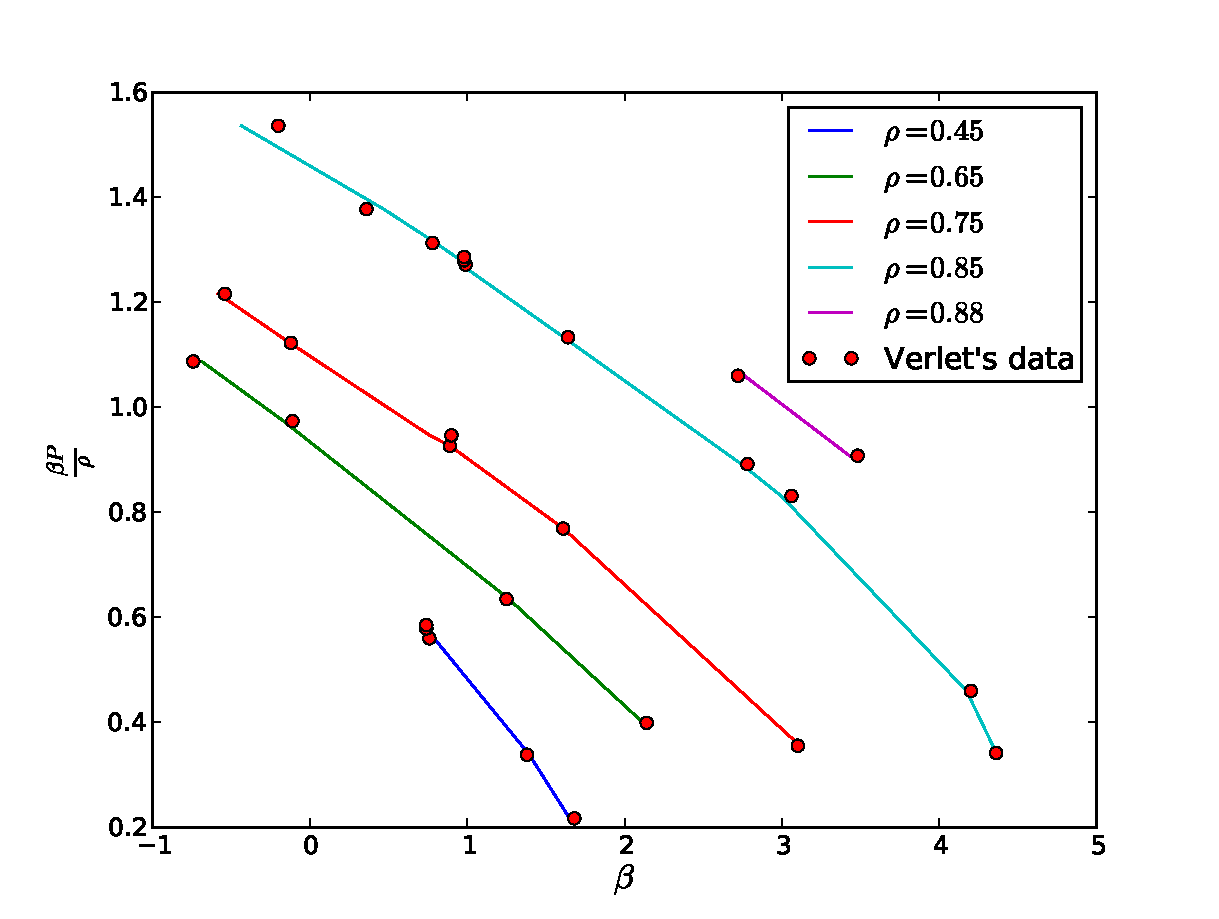
\includegraphics[height=80mm]{P.pdf}
  \caption[]{The compressibility factor $\beta P/\rho$ as a function of $\beta$ for isochores $\rho=0.88$, 0.85, 0.75, 0.65 and 0.45 (solid colored lines), and compared with the data computed by Verlet \citep{PhysRev.159.98}. The red dots that overlap with the lines correspond to measurements of the same density.}
  \label{fig:pressure}
\end{figure}

In figure \ref{fig:cv} the results of the measurements of the specific heat are plotted as a function of temperature. The data corresponds to what we would expect in high density, low temperature and low density, high temperature situations, respectively the Dulong\text{-}Petit law and the specific heat for a ideal gas at high temperature. The errors are in the order of 50 to 100.\\ 

\begin{figure}[!htb]
  \centering
    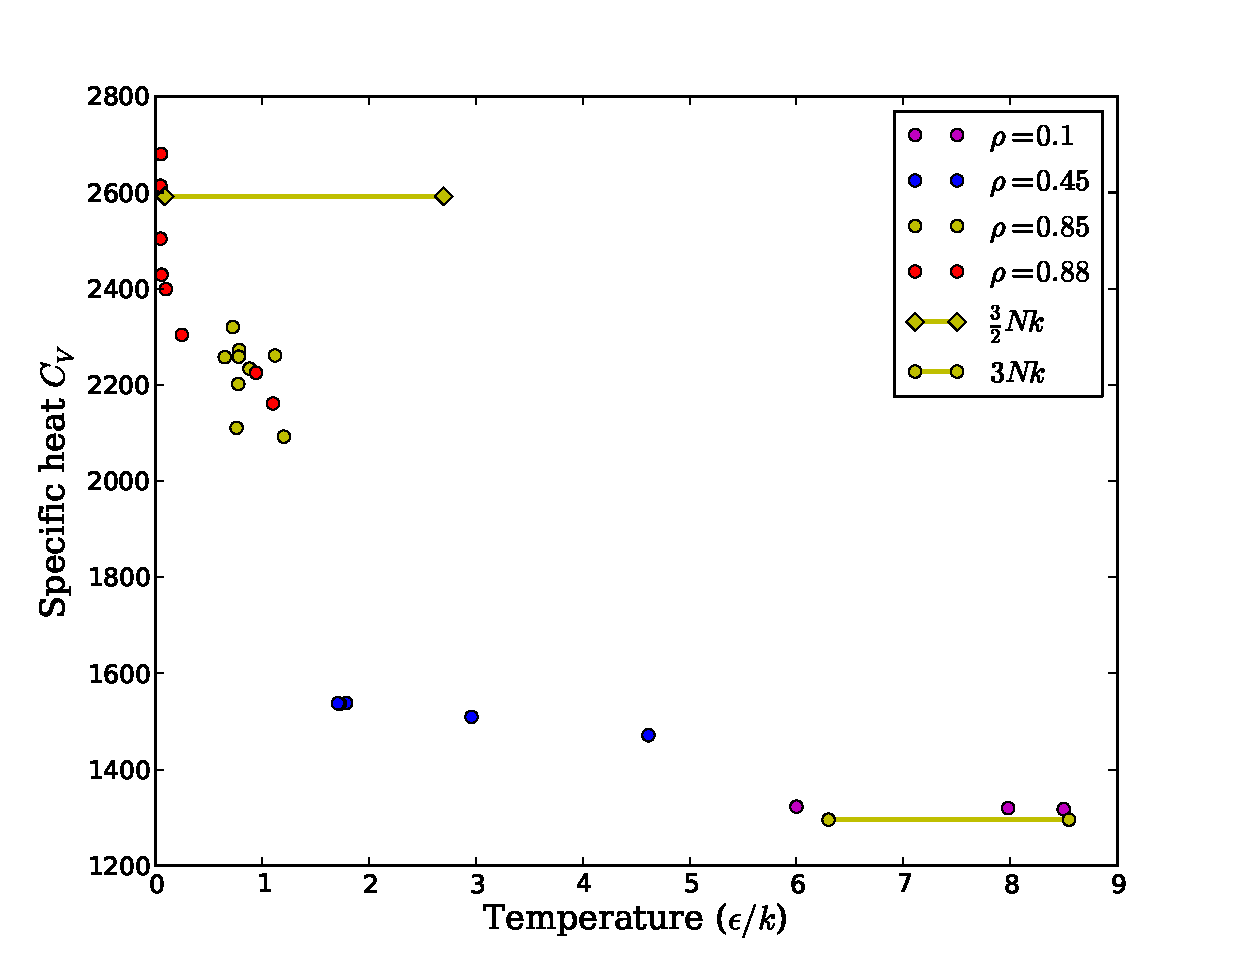
\includegraphics[height=70mm]{cv.pdf}
  \caption[]{The specif heat as a function of temperature. The specific heat that we expect at high density, low temperature and low density, high temperature systems, respectively the Dulong\text{-}Petit law and the specific heat for a ideal gas at high temperature are similar to what is measured.}
  \label{fig:cv}
\end{figure}

With the method of least squares we calculated the diffusion coefficient $D$ and found a corresponding error of 0.1\%. For $\rho=0.85$ the diffusion coefficient is plotted as a function of temperature and pressure in figure \ref{fig:D}. The diffusion coefficients we measured for other densities can be found in table \ref{tab:label}. \\

\begin{figure}[!htb]
  \centering
    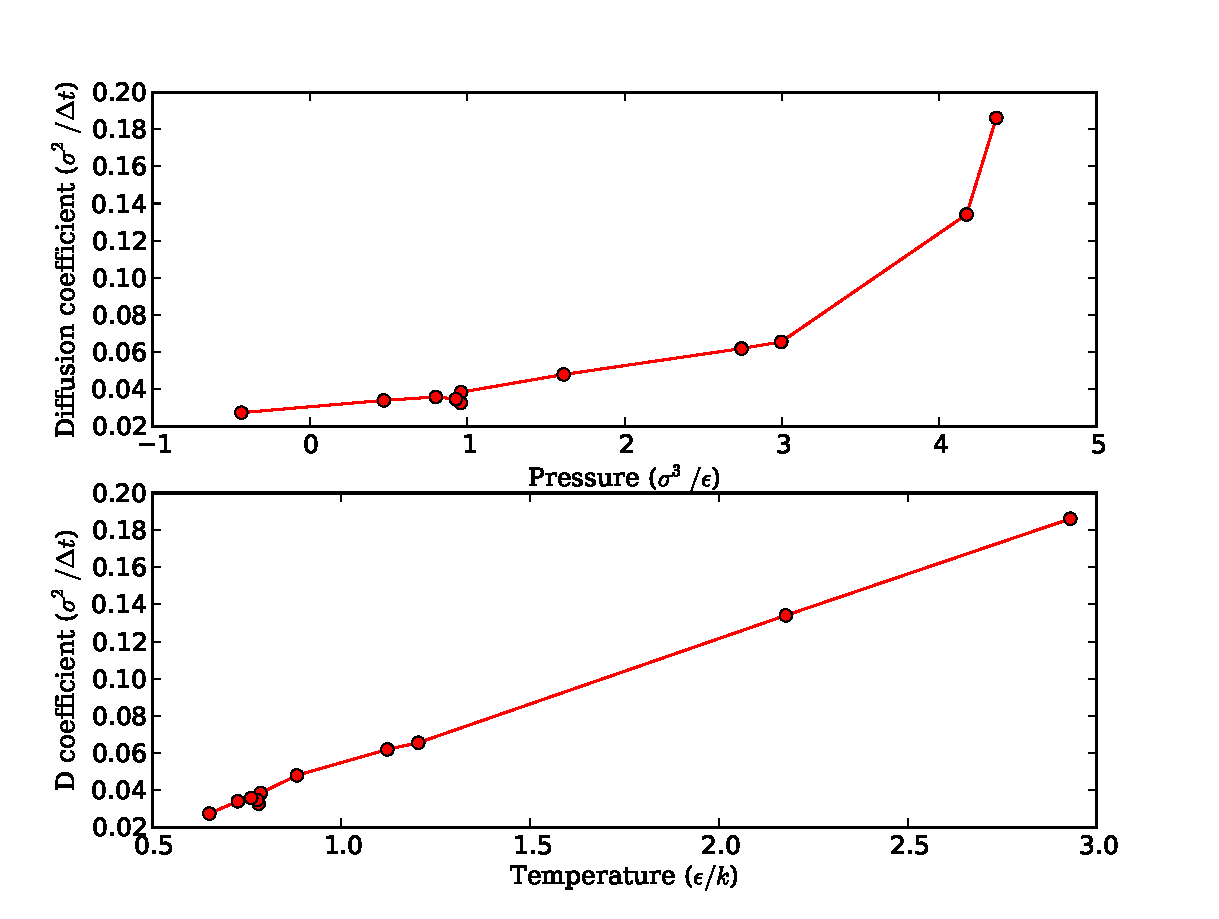
\includegraphics[height=70mm]{D.pdf}
  \caption[]{Diffusion coefficient as a function of pressure (top) and temperature (bottom) for $\rho=0.85$.}
  \label{fig:D}
\end{figure}


The chemical potential we measured can be found in table \ref{tab:label}. The chemical potential goes down very rapid on increasing temperature and consequently pressure. This is what was expected, as it is 'costs' more energy to add a particle to the system. The error in these measurements varies from 3 to 25 \%. \\

\begin{table}[!htb]
\centering
\label{tab:tabel}
\caption{List of thermodynamical results: $\rho$ is the particle density, $T_0$ is the preset temperature, and $T$ is the average temperature of the system, $\beta P/ \rho$ is the compressibility factor, $\mu$ is the chemical potential, $C_V$ is the specific heat and $D$ is the diffusion coefficient. The units can easily be derived from the reduced units given in section \ref{reduced}.}
\begin{tabular}{|l|l|l|l|l|l|l|l|}
\hline
$\rho$ & $T_{0}$ & $T$ & $U$ & $\beta P/ \rho$ & $\mu$ & $C_V$ & $D$\\ \hline
0.45 & 4.63 & 4.62 & 4079 & 1.65 & -1.5584650 & 1471 & 0.844\\ \hline
0.45 & 2.94 & 2.96 & 1629 & 1.39 & -0.5454923 & 1510 & 0.673\\ \hline
0.45 & 1.76 & 1.79 & -156 & 0.79 & -0.1087776 & 1539 & 0.436\\ \hline
0.45 & 1.74 & 1.73 & -245 & 0.75 & -0.0953481 & 1537 & 0.446\\ \hline
0.45 & 1.71 & 1.71 & -281 & 0.71 & -0.0918470 & 1538 & 0.413\\ \hline
0.65 & 2.56 & 2.51 & 20 & 2.12 & -0.1401748 & 1644 & 0.297\\ \hline
0.65 & 1.59 & 1.58 & -1560 & 1.27 & -0.0162097 & 1789 & 0.203\\ \hline
0.65 & 1.04 & 1.03 & -2531 & -0.17 & -0.0009151 & 1825 & 0.136\\ \hline
0.65 & 0.90 & 0.92 & -2731 & -0.69 & -0.0003651 & 1809 & 0.128\\ \hline
0.75 & 2.85 & 2.82 & 209 & 3.11 & -0.1468995 & 1740 & 0.237\\ \hline
0.75 & 1.30 & 1.30 & -2570 & 1.61 & -0.0022013 & 2050 & 0.115\\ \hline
0.75 & 1.07 & 1.08 & -2997 & 0.89 & -0.0004953 & 1856 & 0.099\\ \hline
0.75 & 1.07 & 1.06 & -3046 & 0.76 & -0.0004050 & 1927 & 0.097\\ \hline
0.75 & 0.88 & 0.89 & -3375 & -0.13 & -0.0000787 & 2034 & 0.079\\ \hline
0.75 & 0.83 & 0.82 & -3509 & -0.58 & -0.0000331 & 2005 & 0.068\\ \hline
0.85 & 2.89 & 2.93 & 225 & 4.36 & -0.1187017 & 1916 & 0.186\\ \hline
0.85 & 2.20 & 2.18 & -1238 & 4.17 & -0.0289495 & 1982 & 0.134\\ \hline
0.85 & 1.21 & 1.20 & -3223 & 3.00 & -0.0004889 & 2092 & 0.065\\ \hline
0.85 & 1.13 & 1.12 & -3398 & 2.74 & -0.0002528 & 2261 & 0.062\\ \hline
0.85 & 0.88 & 0.88 & -3927 & 1.61 & -0.0000201 & 2234 & 0.048\\ \hline
0.85 & 0.79 & 0.79 & -4138 & 0.96 & -0.0000050 & 2273 & 0.038\\ \hline
0.85 & 0.78 & 0.78 & -4143 & 0.96 & -0.0000045 & 2259 & 0.033\\ \hline
0.85 & 0.78 & 0.78 & -4154 & 0.93 & -0.0000043 & 2202 & 0.035\\ \hline
0.85 & 0.76 & 0.76 & -4188 & 0.80 & -0.0000033 & 2111 & 0.036\\ \hline
0.85 & 0.72 & 0.73 & -4270 & 0.47 & -0.0000017 & 2320 & 0.034\\ \hline
0.85 & 0.66 & 0.65 & -4448 & -0.43 & -0.0000003 & 2257 & 0.027\\ \hline
0.88 & 1.10 & 1.10 & -3558 & 3.43 & -0.0001595 & 2161 & 0.050\\ \hline
0.88 & 0.94 & 0.94 & -3921 & 2.76 & -0.0000317 & 2225 & 0.039 \\ \hline
\end{tabular}
\label{tab:label}
\end{table}

We can say something about the state of the system by measuring the static pair correlation function (PCF). In figure \ref{fig:pcf} the PCF is plotted as a function of distance to a reference particle for different temperatures. \\

\begin{figure}[htbp]
  \centering
    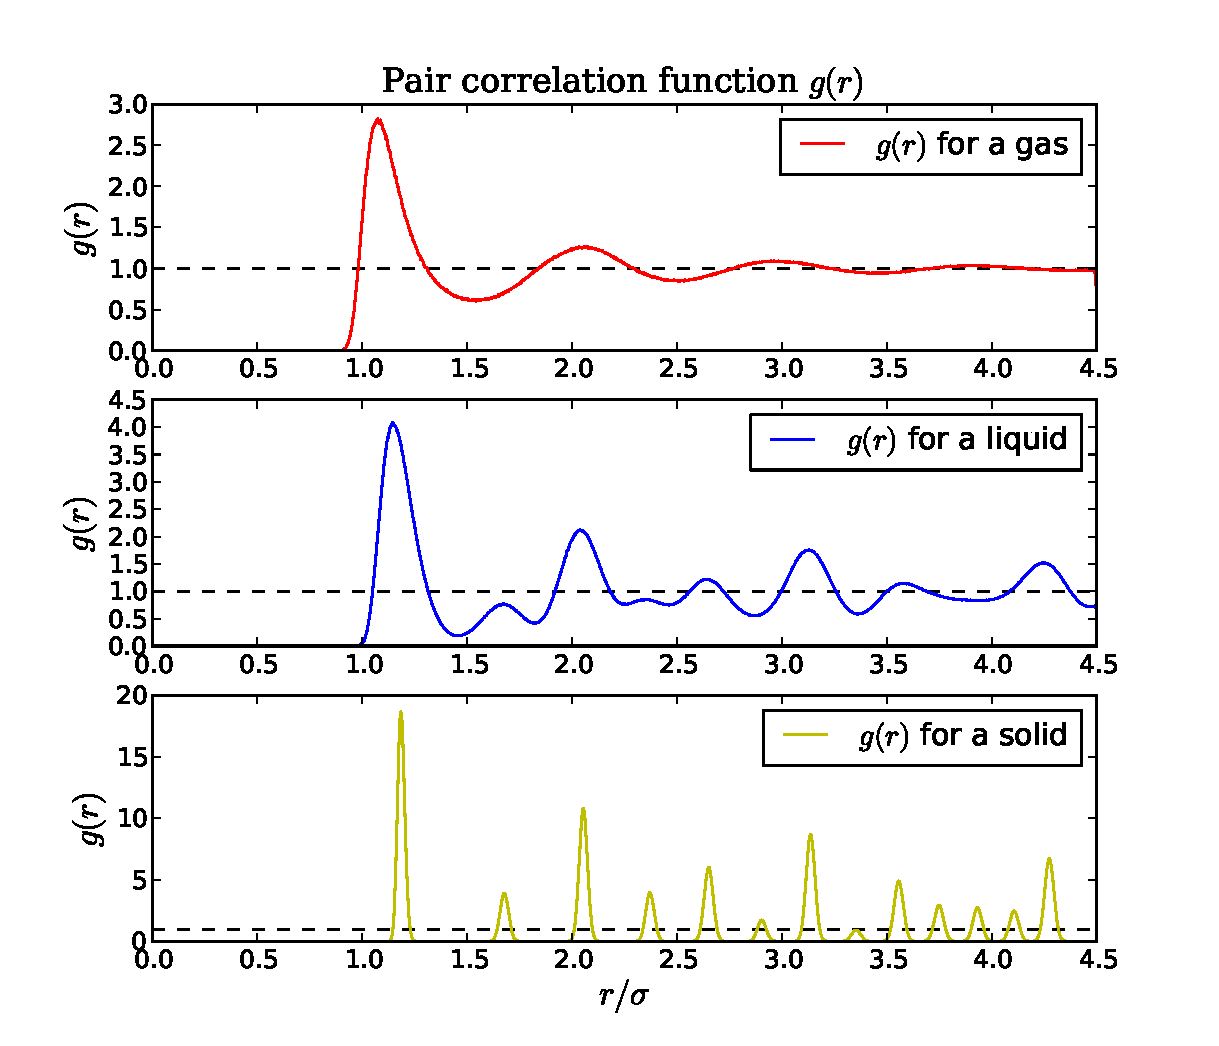
\includegraphics[height=100mm]{pcf.pdf}
  \caption[]{The static pair correlation (PCF) function as a function of distance to a reference particle. In the PCF one can see how many neighbors an particle has, and thus the density around a particle. At the top is a PCF for a gas ($T=1$ and $\rho=0.85$), which has a uniform density after a certain distance. In the middle a PCF for a liquid ($T=0.3$ and $\rho=0.85$) and at the bottom for a solid ($T=0.01$ and $\rho=0.85$). The first peak indicates its 12 nearest neighbors in the fcc and the second peak its 6 next nearest neighbors.}
  \label{fig:pcf}
\end{figure}


\section{Conclusions}
It can be concluded that the Lennard\text{-}Jones potential represents the behavior of argon and with it one can predict the equilibrium properties of argon by integrating relatively easy equations. The striking result \footnote{actually not really surprising, as many others before me did the same thing, but nonetheless...} is the over\text{-}all agreement with experimental data of real argon. 
%----------------------------------------------------------------------------------------
%	BIBLIOGRAPHY
%----------------------------------------------------------------------------------------

\bibliography{mybib}{}
\bibliographystyle{plain}



%----------------------------------------------------------------------------------------

\section{Appendix}
\subsection{Remarks}
It should be noted that I made all the plots in this report myself, and most of them are very dynamic. For example, the boundary condition plot (Fig. \ref{fig:BC}) has as input 'number of particles' and then randomly places the particles and draws the lines. The plot of the autocorrelation function automatically finds the closest value to $1/e$ in the array of the autocorrelation function, and draws the corresponding line. All plots are in vector form and made with the matplotlib library for Python. All of the 'hardcore' calculations are done in Fortran which writes the results to some files. These files are read with a Python program in which all the data analysis is done. I'm sorry for exceeding the four page limit you requested, I got a bit excited...

\subsection{The use of my program}
Attached to this report is a .zip-file that contains my program. The Fortan part is called \emph{md.f90} in which you can edit the input parameters in the first lines. After compiling and running the program with the command: \emph{make; ./md}, four files are created,\emph{data.dat, histogram.dat, mu.dat} and \emph{array.dat}.\\

Open your favorite command shell to run the Python program \emph{an.py} which prints some results. You can then enter the commands:\\ \emph{plot\_pressure(), plot\_pcf(), plot\_energy()}, \emph{plot\_temperature()} or \emph{plot\_autocorrelation()}.\\

In the folder \emph{plots} you can find all the scripts to generate the other plots in this report.


\subsection{Data}
Tables with all the measurements used in the report\footnote{can also be found in \emph{data/data.ods}}.
\begin{center}
\begin{tabular}{llllllll}
Ref. \# & Time steps & $\rho$ & $T_0$ & $T$ & $T$ error & $U$ & $U$ error\\
1 & 10000 & 0.45 & 4.63 & 4.6152 & 0.000693 & 4079.5 & 0.1295\\
2 & 10000 & 0.45 & 2.94 & 2.9597 & 0.000519 & 1628.5 & 0.0738\\
3 & 10000 & 0.45 & 1.76 & 1.7870 & 0.000294 & -156.0 & 0.0266\\
4 & 10000 & 0.45 & 1.74 & 1.7288 & 0.000186 & -244.6 & 0.0277\\
5 & 10000 & 0.45 & 1.71 & 1.7102 & 0.000214 & -281.5 & 0.0337\\
6 & 6000 & 0.65 & 2.56 & 2.5081 & 0.000317 & 19.7 & 0.0799\\
7 & 6000 & 0.65 & 1.59 & 1.5766 & 0.000382 & -1560.5 & 0.0487\\
8 & 8000 & 0.65 & 1.04 & 1.0275 & 0.000203 & -2530.7 & 0.0367\\
9 & 6000 & 0.65 & 0.90 & 0.9200 & 0.000208 & -2730.8 & 0.0234\\
10 & 8000 & 0.75 & 2.85 & 2.8167 & 0.000422 & 208.9 & 0.0761\\
11 & 8000 & 0.75 & 1.30 & 1.3009 & 0.000465 & -2569.9 & 0.0420\\
12 & 8000 & 0.75 & 1.07 & 1.0798 & 0.000249 & -2996.8 & 0.0285\\
13 & 10000 & 0.75 & 1.07 & 1.0570 & 0.000314 & -3046.2 & 0.0230\\
14 & 10000 & 0.75 & 0.88 & 0.8909 & 0.000237 & -3375.2 & 0.0168\\
15 & 10000 & 0.75 & 0.83 & 0.8225 & 0.000136 & -3509.0 & 0.0185\\
16 & 5000 & 0.85 & 2.89 & 2.9298 & 0.000765 & 225.5 & 0.1126\\
17 & 3000 & 0.85 & 2.20 & 2.1766 & 0.000650 & -1237.8 & 0.1391\\
18 & 8000 & 0.85 & 1.21 & 1.2038 & 0.000265 & -3223.1 & 0.0447\\
19 & 3000 & 0.85 & 1.13 & 1.1220 & 0.000241 & -3398.5 & 0.0733\\
20 & 3000 & 0.85 & 0.88 & 0.8826 & 0.000230 & -3926.7 & 0.0645\\
21 & 6000 & 0.85 & 0.79 & 0.7865 & 0.000127 & -4137.6 & 0.0160\\
22 & 6000 & 0.85 & 0.78 & 0.7815 & 0.000264 & -4143.4 & 0.0272\\
23 & 5000 & 0.85 & 0.78 & 0.7776 & 0.000171 & -4154.1 & 0.0215\\
24 & 6000 & 0.85 & 0.76 & 0.7619 & 0.000147 & -4187.6 & 0.0204\\
25 & 10000 & 0.85 & 0.72 & 0.7262 & 0.000176 & -4269.8 & 0.0189\\
26 & 8000 & 0.85 & 0.66 & 0.6511 & 0.000168 & -4447.5 & 0.0342\\
27 & 8000 & 0.88 & 1.10 & 1.1021 & 0.000271 & -3557.8 & 0.0424\\
28 & 8000 & 0.88 & 0.94 & 0.9436 & 0.000295 & -3921.1 & 0.0379
\end{tabular}
\end{center}

\begin{center}
\begin{tabular}{lllllll}
Ref. \# & $P$ & $P$ error & $K$ & $K$ error & $\mu$ & $\mu$ error\\
1 & 1.65 & 0.000098 & 5981.25 & 0.90 & -1.5584650 & 0.0320396\\
2 & 1.39 & 0.000069 & 3835.75 & 0.67 & -0.5454923 & 0.0131166\\
3 & 0.79 & 0.000034 & 2315.93 & 0.38 & -0.1087776 & 0.0045889\\
4 & 0.75 & 0.000027 & 2240.56 & 0.24 & -0.0953481 & 0.0046138\\
5 & 0.71 & 0.000036 & 2216.39 & 0.28 & -0.0918470 & 0.0037221\\
6 & 2.12 & 0.000141 & 3250.51 & 0.41 & -0.1401748 & 0.0076038\\
7 & 1.27 & 0.000065 & 2043.34 & 0.50 & -0.0162097 & 0.0012737\\
8 & -0.17 & 0.000233 & 1331.66 & 0.26 & -0.0009151 & 0.0001072\\
9 & -0.69 & 0.000376 & 1192.29 & 0.27 & -0.0003651 & 0.0000557\\
10 & 3.11 & 0.000318 & 3650.43 & 0.55 & -0.1468995 & 0.0091052\\
11 & 1.61 & 0.000220 & 1686.01 & 0.60 & -0.0022013 & 0.0002915\\
12 & 0.89 & 0.000025 & 1399.38 & 0.32 & -0.0004953 & 0.0000713\\
13 & 0.76 & 0.000071 & 1369.90 & 0.41 & -0.0004050 & 0.0000660\\
14 & -0.13 & 0.000301 & 1154.58 & 0.31 & -0.0000787 & 0.0000137\\
15 & -0.58 & 0.000268 & 1065.95 & 0.18 & -0.0000331 & 0.0000059\\
16 & 4.36 & 0.000884 & 3797.07 & 0.99 & -0.1187017 & 0.0077077\\
17 & 4.17 & 0.000947 & 2820.82 & 0.84 & -0.0289495 & 0.0026262\\
18 & 3.00 & 0.000434 & 1560.11 & 0.34 & -0.0004889 & 0.0000745\\
19 & 2.74 & 0.000381 & 1454.13 & 0.31 & -0.0002528 & 0.0000422\\
20 & 1.61 & 0.000156 & 1143.79 & 0.30 & -0.0000201 & 0.0000034\\
21 & 0.96 & 0.000006 & 1019.37 & 0.16 & -0.0000050 & 0.0000012\\
22 & 0.96 & 0.000014 & 1012.79 & 0.34 & -0.0000045 & 0.0000011\\
23 & 0.93 & 0.000016 & 1007.82 & 0.22 & -0.0000043 & 0.0000009\\
24 & 0.80 & 0.000038 & 987.39 & 0.19 & -0.0000033 & 0.0000008\\
25 & 0.47 & 0.000128 & 941.19 & 0.23 & -0.0000017 & 0.0000005\\
26 & -0.43 & 0.000374 & 843.80 & 0.22 & -0.0000003 & 0.0000001\\
27 & 3.43 & 0.000604 & 1428.26 & 0.35 & -0.0001595 & 0.0000255\\
28 & 2.76 & 0.000548 & 1222.85 & 0.38 & -0.0000317 & 0.0000059
\end{tabular}
\end{center}

\begin{center}
\begin{tabular}{lllllll}
Ref. \# & $C_V$ & $t_{eq}$ & $P_{verlet}$ & $\Delta t$ & $D$ & $D$ error\\
1 & 1471 & 6000 & 1.68 & 0.004 & 0.8440 & 0.0247\\
2 & 1510 & 6000 & 1.38 & 0.004 & 0.6730 & 0.0136\\
3 & 1539 & 6000 & 0.76 & 0.004 & 0.4362 & 0.0093\\
4 & 1537 & 6000 & 0.74 & 0.004 & 0.4460 & 0.0080\\
5 & 1538 & 6000 & 0.74 & 0.004 & 0.4133 & 0.0142\\
6 & 1644 & 3000 & 2.14 & 0.004 & 0.2969 & 88.0962\\
7 & 1789 & 3000 & 1.25 & 0.004 & 0.2028 & 53.4799\\
8 & 1825 & 6000 & -0.11 & 0.004 & 0.1358 & 31.4946\\
9 & 1809 & 3000 & -0.74 & 0.004 & 0.1278 & 20.0718\\
10 & 1740 & 5000 & 3.1 & 0.004 & 0.2367 & 0.0040\\
11 & 2050 & 5000 & 1.61 & 0.004 & 0.1147 & 0.0030\\
12 & 1856 & 5000 & 0.89 & 0.004 & 0.0993 & 0.0024\\
13 & 1927 & 5000 & 0.9 & 0.002 & 0.0974 & 0.0056\\
14 & 2034 & 5000 & -0.12 & 0.002 & 0.0787 & 0.0016\\
15 & 2005 & 5000 & -0.54 & 0.002 & 0.0683 & 0.0022\\
16 & 1916 & 500 & 4.36 & 0.004 & 0.1862 & 0.0134\\
17 & 1982 & 500 & 4.2 & 0.004 & 0.1341 & 0.0072\\
18 & 2092 & 3000 & 3.06 & 0.004 & 0.0655 & 0.0046\\
19 & 2261 & 500 & 2.78 & 0.004 & 0.0619 & 0.0031\\
20 & 2234 & 500 & 1.64 & 0.004 & 0.0479 & 0.0027\\
21 & 2273 & 1500 & 0.99 & 0.004 & 0.0383 & 0.0039\\
22 & 2259 & 1500 & 0.98 & 0.004 & 0.0326 & 0.0019\\
23 & 2202 & 1000 & 0.98 & 0.004 & 0.0346 & 0.0032\\
24 & 2111 & 2000 & 0.78 & 0.004 & 0.0358 & 0.0021\\
25 & 2320 & 6000 & 0.36 & 0.003 & 0.0339 & 0.0010\\
26 & 2257 & 3000 & -0.2 & 0.004 & 0.0273 & 0.0033\\
27 & 2161 & 5000 & 3.48 & 0.004 & 0.0505 & 0.0015\\
28 & 2225 & 5000 & 2.72 & 0.004 & 0.0385 & 0.0015
\end{tabular}
\end{center}



\end{document}